\documentclass{article}
\usepackage[utf8]{inputenc}
\usepackage{times}
\usepackage{graphicx}
\usepackage[margin=1in]{geometry}
\usepackage{hyperref}
\renewcommand{\baselinestretch}{1.5}

\author{Bijan Varjavand}
\title{Microstructure and Crystal Structure\\Groub 2d}

\begin{document}

\maketitle
\ \\[2.5in]

\section{Abstract}
The lab mainly focused on two tasks, both focused on samples of As-Received Steel and Aluminum, and annealed Steel and Aluminum. The first task was to polish and view samples, calculating the average grain sizes manually and compare them with computer-generated values. Manually, using the ASTM standard, the grain number for transverse 1018 as received steel was measured to be 8.86 ($252 \mu m^2$), while the grain number for the longitudinal orientation was 8.86 ($356 \mu m^2$). The LAS V.4 calculated grain numbers for transverse as 8.65 ($356 \mu m^2$) and 9.25 ($252 \mu m^2$) for the longitudinal side. Digital results for annealed Steel showed smaller grain numbers in both orientations, indicating less Hall-Petch strengthening as expected. The second task was to perform x-ray diffraction analysis on annealed 1018 steel and aluminum 6061. This was accomplished through deriving Bragg's law and using it as a tool to solve for interplanar spacing values. The lattice parameter for annealed 6160 Al is 0.405nm, and the lattice parameter for annealed 1018 steel is 0.28nm.

\clearpage

\section{Introduction}

\subsection{The Unit Cell}

The unit cell has multiple different conformations. Examples include body-centered cubic(BCC)(\textbf{Fig1}) and face-centered cubic(FCC)(\textbf{Fig1}).

\begin{figure}[h]
	\begin{minipage}{0.5\textwidth}
		\centering
		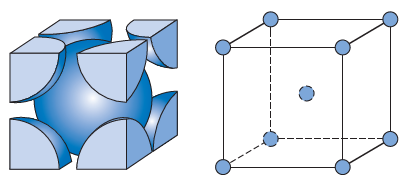
\includegraphics[scale=.7]{bcc.png}
	\end{minipage}
	\begin{minipage}{0.5\textwidth}
		\centering
		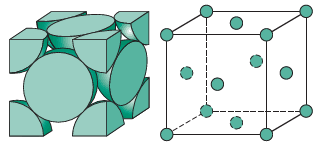
\includegraphics[scale=.85]{fcc.png}
	\end{minipage}
	\caption{Left: BCC, Right: FCC}
\end{figure}

One important aspect of a unit cell is its burgers vector and dense plane. These values indicate the direction of most dense packing. Notation for these dense direction is in miller indices (h, k, l, where hkl are orthogonal directional axes). Not only that, but due to symmetry of unit cells, the burgers vector is a family of h, k, and l values. For example, the family \{1 1 0\} includes all hkl values that, when squares are added, equal 1. This is actually the burgers vector for FCC unit cells, and a one is shown below.

\begin{figure}[h]
	\centering
	\includegraphics[scale=.85]{"dense direction".png}
	\caption{Dense plane for FCC unit cell - \{1 1 0\}}
\end{figure}

One can see that, in the unit cell space, the "dense direction" is easily found as the highest density of atoms in a specific direction(\textbf{Fig2}). This is also the direction that slips form across most easily due to the close stacking of atoms. This is due to stacking fault energy in that direction being the lowest, as the maximum displacement between atoms is lowest(due to distance between atoms being the lowest as well).

\ 

Dislocations are linear imperfections in a crystal structure, and occur along the Burgers vector. The more dislocations are present in a material, the more difficult it is for the material to be bent and shaped. This is due to the dislocations.

\subsection{Grain Boundaries} 

The orientation of h, k, and l vectors are linked to each other within each grain(\textbf{Fig3}). At the grain boundary, dislocation lines separate the slight change in orientation of h, k, and l vectors. These lines are visible to optical microscopy and can be counted - exactly the contents of this section of the lab. A fundamental diagram of grain boundaries is seen below

\begin{figure}[h]
	\centering
	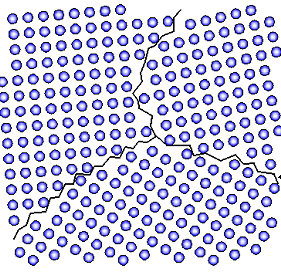
\includegraphics[scale=1.5]{grain.png}
	\caption{black lines are the dislocations separating grains. \url{<http://www.engineeringarchives.com/img/les\_ matsci_surfacedefects_1.png>}}
\end{figure}

An important quality of grain boundaries to note is that the strength of the material is inversely proportional to grain size. 
This is because the grain boundaries block dislocations from traveling. The specific strengthening mechanism is known as Hall-Petch strengthening. Influencing dislocation movement also influences yield strength and thus the strength of the material.

\subsection{Our Samples}

Specifically, the samples that were used include as received steel 1018, annealed steel 1018, and titanium 6-4. We also observed the x-ray diffraction pattern of aluminum 6061. Discussion of the importance of each sample is important for understanding the scope of the lab.

The 1018 in 1018 steel is from the composition of the material. It is made of 0.18\% Carbon, 0.6-0.9\% Manganese, and 98.82-99.22\% Iron. Due to its low carbon content, it has good weldability and a good balance of toughness, strength, and ductility. It is used in a huge variety of applications, including most casting processes.

Titanium 6-4 has a more complicated composition, but the notable elements are Aluminum(6\%) and Vanadium(4\%). The main use for these materials is in cogs among other applications due to their high toughness and tensile strength even at high temperatures. They also have a low weight. Additionally, there are uses for this material in the biomedical field due to its low weight and compatibility with bone and tissue.

Aluminum 6061 is composed of Aluminum, Magnesium, Silicon, Manganese, and Chromium, while the 6061 is from the 0.60\% weight percent in the specific alloy. One use for this material is in bicycle frames due its extremely low weight. One notable feature of aluminum and its alloys are difficult to anneal, since they will melt almost immediately. One technique to assist in annealing is to leave soap on the material as it will turn black under heat almost immediately, indicating success of the annealing process.

\subsection{Optical Microscopy}

Optical microscopy is a technique that uses light to view the sample at high magnification. The main method of generating images at such high magnifications are the use of multiple magnifying lenses as well as a light source

Preparing my samples to be viewed by the optical microscope was not trivial. The first step after acquiring my sample was to polish it. The complexity with polishing is that one can't use a grit that is too low or high. At each step, you just erase the scratches you made with the coarser grit with finer and smaller scratches - eventually they become too small to see.

Etching must be done afterwards in order to make the grain boundaries noticeable. This is done by reacting the sample with an organic material - the reaction with the grains of the sample make them prominent and visible.

\subsection{X-Ray Diffraction}

X-Ray diffraction is a useful tool for finding crystalline features, utilizing Bragg's law which relates interatomic spacing, interplanar spacing, and miller indices, with the path length of the incident beam to the refracted beam. Deriving this law can be done by analyzing the diagram below - an example for the physical process in x-ray diffraction.

\begin{figure}[h]
	\centering
	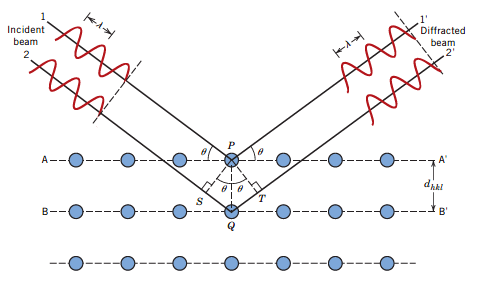
\includegraphics[scale=1]{bragg.png}
	\caption{A diagram of x-ray diffraction}
\end{figure}

We can see that the crucial line segment is PQ, as it equals $d_{hkl}$, the interplanar spacing(\textbf{Fig4}). You can calculate $d_{hkl}$. Derivation is as follows
$$n\lambda = SQ + QT$$
$$n\lambda = d_{hkl}sin(\theta ) + d_{hkl}sin(\theta )$$
$$n\lambda = 2d_{hkl}sin(\theta ), = Bragg's\ Law$$
The interplanar spacing, $d_{hkl}$, is actually dependent on the miller indices and lattice parameter a. We can see below
$$d_{hkl} = \frac{a}{\sqrt{h^2+k^2+l^2}}$$
Combining these equations, we get
$$a = \sqrt{\frac{\lambda ^2}{4*sin(\theta)^2}(h^2+k^2+l^2)}$$.
The basic rules for h,k, and l values depend on the dense planes of the material, which depend on the crystal structure of the material. For BCC structures, h+k+l must be an even number in order for diffraction to occur. For FCC structures, h, k, and l must all be even or odd.
This is the basis for how values were generated from the data.

\section{Procedure}

\subsection{1A}

The first step was to organize the samples. The group labeled the transverse orientation and longitudinal orientation for the 2 1018 steel samples. After manually sanding the samples and creating epoxy pucks, the machine began its automated polishing protocol. The machine used SIC Foil \#220 for 2:20 minutes, and then used MD Largo 9$\mu$m, MD Reic 3$\mu$m, Md-Nap 1$\mu$m polishing plates with the associated settings and lubricants. The lubricants used were water, eventually reaching diamond-particles of smaller and smaller sizes, eventually reaching $1\mu$m. Once the samples were polished completely, they were etched with Nitol for 30 seconds. This allowed the grains to become distinguishable from each other. The samples were then viewed on the optical microscope. After locating a clean spot on the sample and focusing the image at 50x, we used the LAS 4.7 grain expert function(specifically avoiding scratching among other defects). For all of our grain expert calculations, we used a sensitivity of 6. We measured the grain sizes of the 1018 annealed steel, the 1018 as-received steel, and the Ti 6-4 sample.

\subsection{X-Ray Diffraction}

A sample of Ti 6-4 was already prepared in the x-ray diffractometer. The TA wore a ring while confirming the state of the sample in order to confirm safe levels of radiation exposure. Data was collected across a range of angles. Specifically the machine ran from $5^o$ to $100^o$ in steps of $0.2^o$. Data for annealed 1018 steel and annealed 6061 aluminum was provided. The wavelength used for all data collection was 0.154nm. Data collected included crystal structure, planes, and planar spacing for all phases. The TA provided XRD data for 1018 annealed steel and 6061 annealed Al.

\section{Results and Discussion}

\subsection{Grain Size}

The group recorded data for longitudinal and transverse 1018 steel (annealed and non-annealed) as well as Ti 6-4. Since I am only analyzing the steel, I will only include the steel images(\textbf{Fig5}). The images for Ti6-4 can be found in the "Lab1" folder in my github repository. This is because the titanium images were deemed too dirty to use. We also only found grain size manually for the as-received steel, as per instructions in the lab report.

\begin{figure}[h]
	\begin{minipage}{0.5\textwidth}
		\centering
		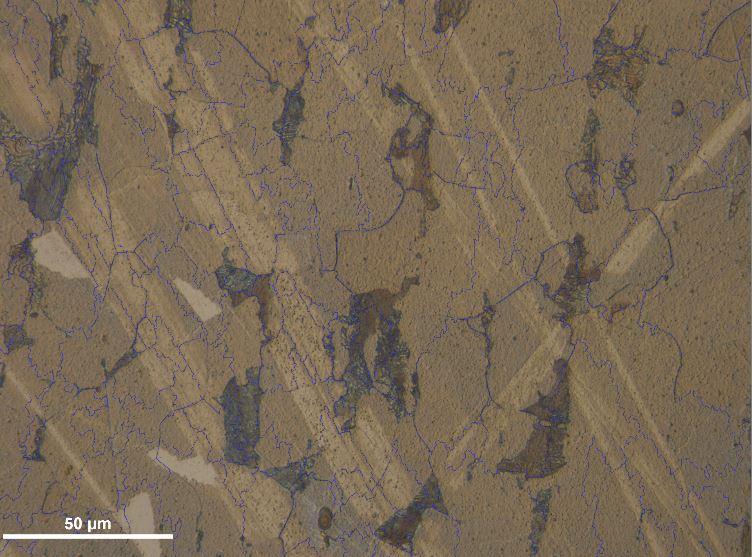
\includegraphics[scale=.35]{LASteelGrains.jpg}
	\end{minipage}
	\begin{minipage}{0.5\textwidth}
		\centering
		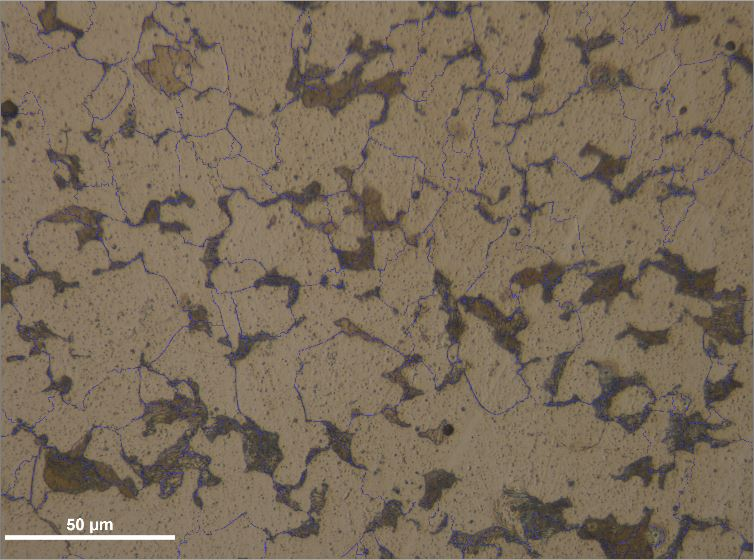
\includegraphics[scale=.35]{TASteelGrains.jpg}
	\end{minipage}\\
	\begin{minipage}{0.5\textwidth}
		\centering
		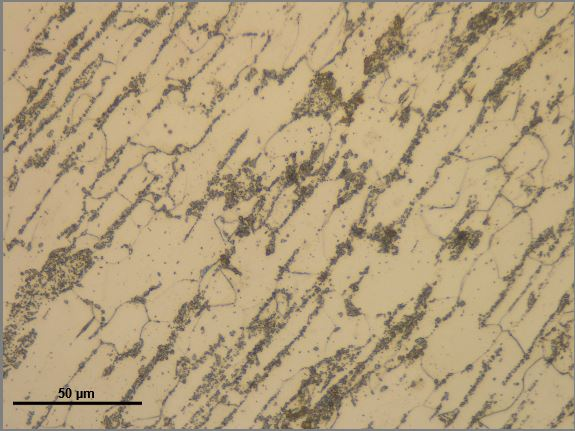
\includegraphics[scale=.46]{LARSteelGrains.jpg}
	\end{minipage}
	\begin{minipage}{0.5\textwidth}
		\centering
		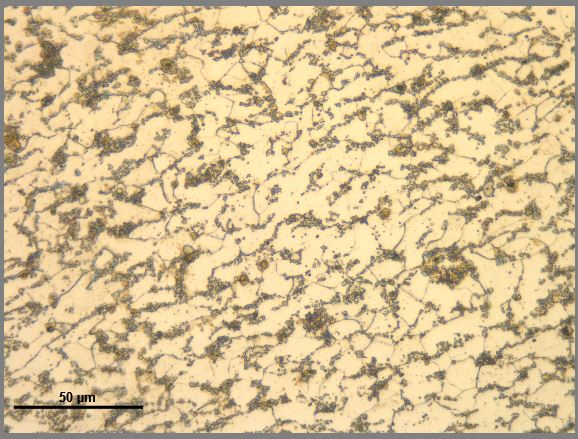
\includegraphics[scale=.46]{TARSteelGrains.jpg}
	\end{minipage}
	\caption{Longitudinal Annealed, Transverse Annealed, then Longitudinal As Received, Transverse As Received}
\end{figure}

Not only did the software save the images, but it also automatically calculated grain size of the samples.

I used the ASTM standard E 112-96 to find grain size manually. The first step to manually count the grain size is to draw four 15cm lines, and then count the number of grains along each line. Four lines are needed because there must be at least 50 grains to reduce noise in the calculations. The average was then found. Then the scale of the image was normalized, using the scale bar found, to obtain the actual size of the grains. This is done by dividing the average per 15cm by the normalization, then converting to mm. Then, the value is plugged into the G equation shown below.
$$G = -3.2877+6.439*log_{10}(N_l)$$
A table was created depicting the values generated as well as values found during manual calculations. Our average grain size for annealed steel samples were only found digitally: Longitudinal annealed steel-9.25, Transverse annealed steel-8.65.


\centering
\begin{tabular}{|| c | c | c | c | c | c | c | c | c ||}
 \hline
 \ & Line1 & Line2 & Line3 & Line4 & Average & $N_l$ & G & computer G\\
 \hline
 \hline
 Longitudinal Steel As Received & 19 & 17 & 15 & 20 & 17.75 & 80.47 & 8.98 & 9.59\\
 \hline
 Transverse Steel As Received & 18 & 19 & 16 & 15 & 17 & 77.07 & 8.86 & 10.46\\
 \hline
\end{tabular}
\raggedright

Where G is the mean grain size.

\ 

The grain size number of 8.98 for longitudinal steel is equal to an average grain area of 252 $\mu m^2$, compared to the value the computer generated of 9.59 $\rightarrow$ 178 $\mu m^2$. The values for transverse steel were manually 8.86 $\rightarrow 252 \mu m^2$ and computer generated 10.46 $\rightarrow 89.1 \mu m^2$.

One can see that grain size is similar for both transverse and longitudinal. This conclusion is somewhat difference in the computer-generated number. The computer's values are both higher than our found values, which imply that visually counting grains makes it easy to skip over the hard-to-see grain boundaries. The results imply that as-received steel 1018 has isotropic behavior in terms of properties related to grain size. Since grain size number is inversely proportional to size of the grains, we can see that the as-received steel has smaller grains than the annealed steel(digitally found to be 358 trans. and 252 long. $\mu m^2$). This implies that 1018 as-received steel is stronger than 1018 annealed steel due to smaller grains and the associated Hall-Petch strengthening from it.

The potential systematic errors are all in the way that the software calculates grain boundaries. This includes the bright field setting we were on, as well as the sensitivity level that we set-which was user bias. Random error includes the specific part of the material that we looked at(the quality of the image, in terms of precipitates as well as polishing artifacts). We were unable to do these measurements for Ti 6-4 since the sample had too severely corroded.

\ 

Taking a look at the hypereutectoid will give us an idea of the degree of faceting on the surface of the material(\textbf{Fig6}). The silicon precipitate is shown in red.

\begin{figure}[h]
	\centering
	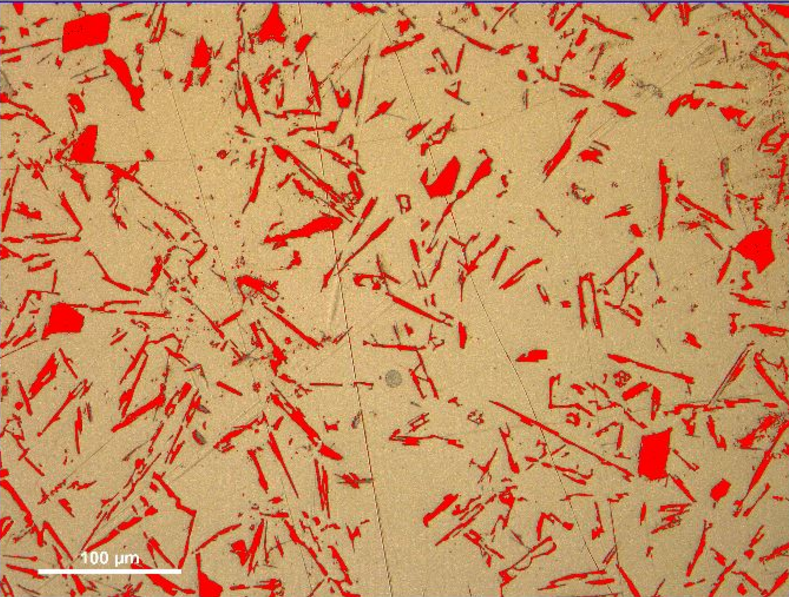
\includegraphics[scale=.6]{hyperu.png}
	\caption{The computer's automated grain size calculator, using the ASTM Standard, E112-96}
\end{figure}

The calculated surface area percentage of the silicon was 11.5\%. This is within the expected amount of 8-12\%.

\subsection{X-Ray Diffraction}

X-ray diffraction data is significant because we can derive interplanar spacing, interatomic spacing, and miller indices from the exhibited peaks in the data.

\begin{figure}[h]
	\begin{minipage}{.5\textwidth}
		\centering
		\includegraphics[scale=.11]{SteelXRD.jpg}
	\end{minipage}		
	\begin{minipage}{.5\textwidth}
		\centering
		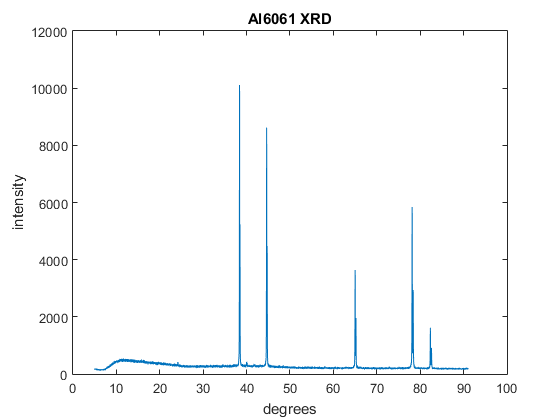
\includegraphics[scale=.6]{ALXRD.png}
	\end{minipage}
	\caption{Left: 1018 annealed steel Right: annealed Aluminum 6061}
\end{figure}

The graphs indicate which hkl values correlate to which high intensity peaks. These peaks are generated from the scattering of light at specific angles, shown below(\textbf{Fig7}). Since we know the crystal structure of steel(BCC) and aluminum(FCC), we can determine beforehand the hkl values for the highest density peaks. This is because they are the dense directions of the material. Once the appropriate miller indices are found, interplanar and interatomic spacing can be solved for. The procedure of determining values for interplanar spacing based off of the data is shown below

$$a = \sqrt{\frac{\lambda ^2}{4*sin(\theta)^2}(h^2+k^2+l^2)}$$
For steel, we know that the dense direction is the \{1 1 0\} family, so the highest peak has an $h^2+k^2+l^2$ value of 2.  Showing the work for the largest peak in iron, and then listing the rest in a table below,
$$a = \sqrt{\frac{2*0.154^2}{4*sin(22.5)^2}} = 0.2846$$
$$d_{hkl} = \frac{0.2846}{\sqrt{2}} = 0.2012$$

\begin{figure}[h]
	\begin{minipage}{0.5\textwidth}
		\centering
		Steel
		
		\begin{tabular}{|| c | c | c | c ||}
		 \hline
		 $2\theta$ & a(nm) & $d_{hkl}$(nm) & Miller Indices\\
		 \hline
		 \hline
		 45 & 0.2846 & 0.2012 & \{1 1 0\}\\
		 \hline
		 65 & 0.2866 & 0.1433 & \{2 0 0\}\\
		 \hline
		 82 & 0.2875 & 0.1174 & \{2 1 1\}\\
		 \hline
		 98.5 & 0.2875 & 0.1016 & \{2 2 0\}\\
		 \hline
		\end{tabular}
	\end{minipage}
	\begin{minipage}{0.5\textwidth}
		\centering
		Aluminum
		
		\begin{tabular}{|| c | c | c | c ||}
		 \hline
		 $2\theta$ & a(nm) & $d_{hkl}$(nm) & Miller Indices\\
		 \hline
		 \hline
		 38.37 & 0.4058 & 0.2343 & \{1 1 1\}\\
		 \hline
		 44.62 & 0.4057 & 0.2028 & \{2 0 0\}\\
		 \hline
		 65.02 & 0.4052 & 0.1433 & \{2 2 0\}\\
		 \hline
		 78.15 & 0.4051 & 0.1222 & \{3 1 1\}\\
		 \hline
		 82.34 & 0.4052 & 0.1670 & \{2 2 2\}\\
		 \hline
		\end{tabular}
	\end{minipage}
\end{figure}

You can see that the a value is similar across all values of $\theta$. This is expected, since interplanar spacing in these materials is constant. The literature values for lattice parameters of annealed 1018 steel and 6061 Al are 0.405 and 0.287 nm, very close to what was calculated.

The main error associated with these data points is the noise from the machine. Systematically, it could be due to wavelength of light used and peak calibration and noise reduction settings. Another would be setting the angular step size. Human error is inherent in the setting of the sample. Some random error is possible - if there was a significant enough disturbance. The small noise in the data (broad peak in aluminum data) was due to peaks found in silicon - this is due to the sample not mounted completely flush, and the incident beam hitting part of the silicon mount as well as the sample.

\end{document}